\documentclass[sigconf,anonymous,review]{acmart}

\usepackage[normalem]{ulem}
\usepackage{amssymb}
\usepackage{amsmath}
\usepackage{algorithm} % environment for the algorithm code (like figure and table)
\usepackage{algorithmicx} % write the pseudo code
\usepackage[noend]{algpseudocode} % layout of the pseudo code
\usepackage{tikz} % needed for: tikz pics
\usepackage{xcolor}
\usepackage{xspace}
\usepackage{natbib}
\usepackage{graphicx}
\usepackage{subfigure}
%\usepackage[inline]{enumitem}

\newcommand{\TODO}[1]{{\bf \em \textcolor{red}{TODO: #1}\xspace}}

\newcommand{\todo}[2]{\textcolor{red}{$\bullet$ \textbf{Task:} #1; \textbf{Responsible:} #2}}

\newcommand{\sys}{VIPRE\xspace}
\newcommand{\sysfull}{Virtualized Intermittently-Powered Runtime Environment\xspace}

\setcopyright{rightsretained}

\acmDOI{http://dx.doi.org/xx.xxxx/xxxxxxx.xxxxxxx}

\acmISBN{978-1-xxxx-xxxx-x/17/11}

\acmConference[ASPLOS]{The 23rd ACM International Conference on Architectural Support for Programming Languages and Operating Systems}{March 24--28, 2017}{Williamsburg, VA, USA}

\acmYear{2017}

\copyrightyear{2017}

\acmPrice{15.00}

\begin{document}

\title[VIPRE: Virtualized Intermittently-Powered Runtime Environment]{VIPRE: Virtualized Intermittently-Powered Runtime Environment}

%Note: order of authors placed randomly

\author{Kiwan Maeng}
%\authornote{}
%\orcid{}
\affiliation{%
	\institution{Carnegie Mellon University}
	\streetaddress{4720 Forbes Avenue}
	\city{Pittsburgh} 
	\state{PA} 
	\postcode{15213}
}
\email{kmaeng@andrew.cmu.edu}

\author{Alexei Colin}
%\authornote{}
%\orcid{}
\affiliation{%
	\institution{Carnegie Mellon University}
	\streetaddress{4720 Forbes Avenue}
	\city{Pittsburgh} 
	\state{PA} 
	\postcode{15213}
}
\email{acolin@andrew.cmu.edu}

\author{Brandon Lucia}
%\authornote{}
%\orcid{}
\affiliation{%
	\institution{Carnegie Mellon University}
	\streetaddress{4720 Forbes Avenue}
	\city{Pittsburgh} 
	\state{PA} 
	\postcode{15213}
}
\email{blucia@andrew.cmu.edu}

\author{Amjad Yousef Majid}
%\authornote{}
%\orcid{}
\affiliation{%
	\institution{Delft University of Technology}
	\streetaddress{Mekelweg 4}
	\city{Delft, The Netherlands} 
	\state{Zuid Holland} 
	\postcode{2628\,CD}
}
\email{a.y.majid@tudelft.nl}

\author{Kas{\i}m Sinan Y{\i}ld{\i}r{\i}m}
%\authornote{}
%\orcid{}
\affiliation{%
	\institution{Delft University of Technology}
	\streetaddress{Mekelweg 4}
	\city{Delft, The Netherlands} 
	\state{Zuid Holland} 
	\postcode{2628\,CD}
}
\email{k.s.yildirim@tudelft.nl}

\author{Przemys{\l}aw Pawe{\l}czak}
%\authornote{}
%\orcid{}
\affiliation{%
	\institution{Delft University of Technology}
	\streetaddress{Mekelweg 4}
	\city{Delft, The Netherlands} 
	\state{Zuid Holland} 
	\postcode{2628\,CD}
}
\email{p.pawelczak@tudelft.nl}

\renewcommand{\shortauthors}{A. Y. Majid et al.}

\begin{abstract}
Computation consistency on intermittently-powered devices can be ensured by: (i) checkpointing, where the volatile state of a program is frequently saved to non-volatile memory, or (ii) via tasks, where a programmer splits the code into small idempotent sections. Results so far suggest that a task-based approach performs better than checkpointing. However, existing tasks-based approaches do not adapt to changing energy levels and storage. This makes the code inefficient (when executed on a larger energy buffer than intended) or can potentially completely disable the program (in the opposite case). Therefore, we present \sys: a task-based execution runtime, enabling code portability by means of a new concept of task coalescing. If a code is written for a very small energy buffer, \sys is able to dynamically coalesce these tasks and constructs a bigger (virtual) task to improve execution times. \todo{Provide concrete numbers for improvement}{Amjad} \todo{Provide concrete numbers for checkpointing improvement}{Amjad}
\end{abstract}

% The code below should be generated by the tool at 
%http://dl.acm.org/ccs.cfm Please copy and paste the code instead of the 
%example below. 

\begin{CCSXML}
	<ccs2012>
	<concept>
	<concept_id>10010520.10010553.10010562.10010564</concept_id>
	<concept_desc>Computer systems organization~Embedded 
	software</concept_desc>
	<concept_significance>500</concept_significance>
	</concept>
	<concept>
	<concept_id>10010520.10010575.10010578</concept_id>
	<concept_desc>Computer systems organization~Availability</concept_desc>
	<concept_significance>300</concept_significance>
	</concept>
	<concept>
	<concept_id>10011007.10010940.10010941.10010949.10010957.10010688</concept_id>
	<concept_desc>Software and its engineering~Scheduling</concept_desc>
	<concept_significance>300</concept_significance>
	</concept>
	<concept>
	<concept_id>10011007.10010940.10010941.10010949.10010965</concept_id>
	<concept_desc>Software and its engineering~Communications 
	management</concept_desc>
	<concept_significance>300</concept_significance>
	</concept>
	<concept>
	<concept_id>10011007.10010940.10010971.10010564</concept_id>
	<concept_desc>Software and its engineering~Embedded 
	software</concept_desc>
	<concept_significance>300</concept_significance>
	</concept>
	</ccs2012>
\end{CCSXML}

\ccsdesc[500]{Computer systems organization~Embedded software}
\ccsdesc[300]{Computer systems organization~Availability}
\ccsdesc[300]{Software and its engineering~Scheduling}
\ccsdesc[300]{Software and its engineering~Communications management}
\ccsdesc[300]{Software and its engineering~Embedded software}

\keywords{Energy harvesting, transient operation, operating system}

\maketitle

\section{Introduction}
\label{sec:intro}

%\TODO{VIPER: Virtualised Intermittent Programming model, Execution model, and Runtime environment}
%\TODO{PREVIEW: Programming and Runtime Environment with Virtualised Intermittent Execution Windows}

%%%%%%%%%%%%%%%%%%%%%% IMPORTANT INFO %%%%%%%%%%%%%%%%%%%%%%%%%%%%%%
% SRAM read/write latency is in the order of 8ns 		 [ Intermittent computation without hardware support of programmer intervention]
% FRAM read/write latency is in the orfer of 60ns/100ns  [Texas Instrument MSP430FR573x DataSheet]
%%%%%%%%%%%%%%%%%%%%%%%%%%%%%


Advances in processor efficiency along with the development of
energy-harvesting systems has created a new category of devices that require
neither a battery nor a tethered power
supply~\citep{prasad_comst_2014,lucia_snapl_2017,soyata_csm_2016}. These
devices operate using ambient energy, such as radio frequency
transmissions~\citep{rf_powered_computing_gollakota_2014},
light~\citep{margolies_infocom_2016,margolies_tosn_2016}, and
vibration~\citep{gorlatova_sigmetrics_2014}. Incorporating compute, storage,
sensing, and communication hardware~\citep{wisp5,moo,capybara}, such devices are a
promising technology for use in the Internet of Things~\citep{ku_cst_2016},
in-body~\citep{nadeau_naturebio_2017} and
on-body~\citep{bandodkar_electroanalysis_2015} medical systems, and
energy-harvesting nano-satellites~\citep{kicksat,capybara}.

Energy-harvesting devices create unique challenges because they operate {\em
intermittently} when energy is
available~\citep{hicks_isca_2017,lucia_snapl_2017}. An energy-harvesting device
buffers energy in a small storage capacitor~\citep{gorlatova_tmc_2013,gunduz_commag_2014} and operates when a
threshold amount of energy has accumulated. Harvestable energy sources are low-power (e.g., nW to $\mu$W) compared to a platform's operating
power level (hundreds of $\mu$W to mW). A device operates briefly until it depletes its buffered energy, after which, the device shuts
down and recharges to operate again later---corresponds to {\em intermittent execution model}~\citep{dino,lucia_snapl_2017} composed of
operation-power failure-restart cycles. As an example, recharge times may be
tens of seconds in radio frequency powered medical device~\cite[Fig.
3c]{nadeau_naturebio_2017}.  The recharge and discharge time---which corresponds to the device's inactive and active time---varies with the energy buffering capacitor's~\cite{capybara} and some devices fail and restart operating $\approx$10 to
$\approx$100 times per second~\citep{tan_infocom_2016,mementos,nvp}.  

\begin{wrapfigure}{t!}{0.5\textwidth}
    \centering
    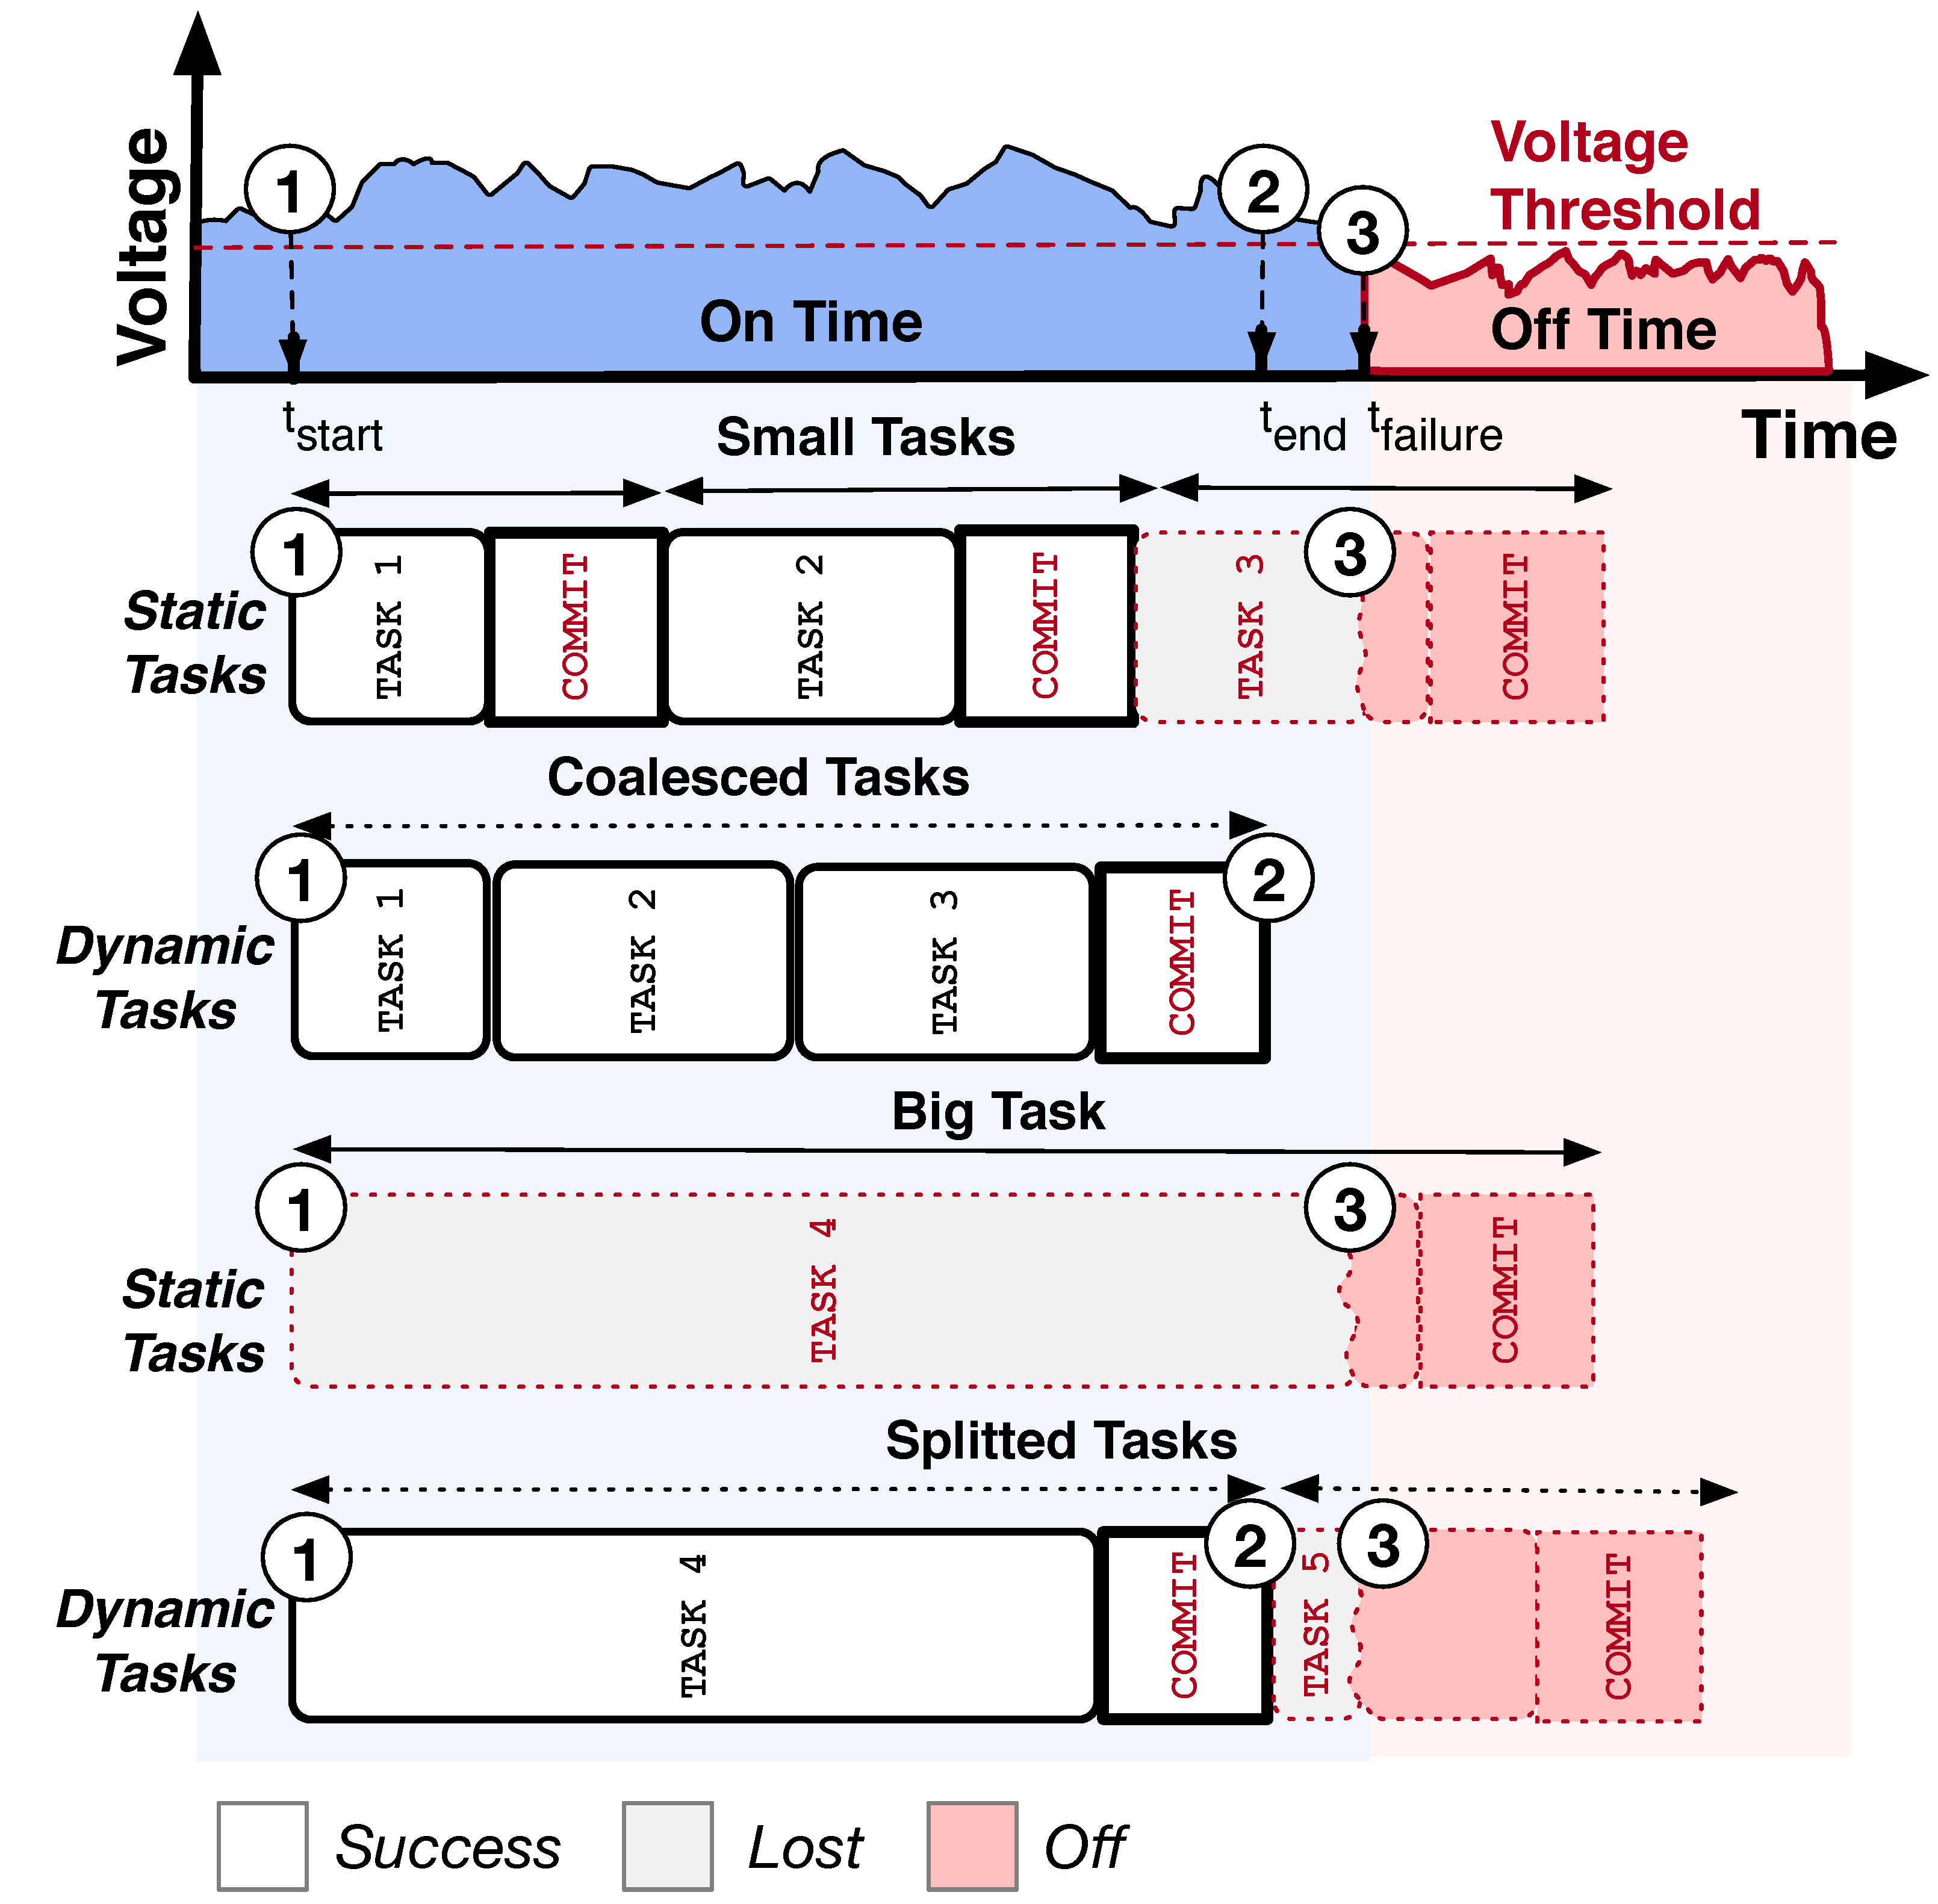
\includegraphics[width=0.5\textwidth]{figures/graffle/intro-figure.pdf}
    \caption{Task coalescing at runtime reduces time and energy overhead in task-based intermittent programming models by performing fewer commits. On the other hand, task splitting reduces wasted computation and enables termination for bigger tasks.}
    \label{fig:coalesce}
\end{wrapfigure}

\textbf{Data Consistency in Intermittent Computing.}  
%Software in an energy-harvesting system operates according to the {\em intermittent execution model}~\citep{dino,lucia_snapl_2017}, which corresponds to the operation-failure-restart cycles of an energy-harvesting device. In an intermittent software execution, an {\em operating period} proceeds for anarbitrary duration (dictated by energy availability) before being interruptedby a {\em failure period}. In a failure period, 
Upon power failures, a device loses the volatile
state in its registers, stack, SRAM, and retains the state of any non-volatile
memory, such as FRAM or Flash. While capturing periodic
checkpoints~\citep{mementos,quickrecall} and sleep
scheduling~\citep{dewdrop,hibernus,hibernusplusplus} help preserve execution
progress, failures can leave non-volatile state incorrectly, partially updated,
and may leave checkpointed volatile state inconsistent with non-volatile state.
These inconsistencies cause intermittent execution to deviate from
continuously-powered behavior, often leading to an unrecoverable
application failure~\citep{dino,edb}. Prior work developed two main approaches to dealing with data inconsistency for
intermittently-powered devices: (i) \emph{software-based programming and
execution models}~\citep{dino,ratchet,chain,alpaca} and (ii)
\emph{hardware-based computer architecture
support}~\citep{hicks_isca_2017,idetic,nvp}.  Complex architectural changes are
expensive to design, verify, and manufacture.  New architectures are also
inapplicable to existing systems~\citep{hicks_isca_2017,nvp}. Software
approaches are simpler and applicable to existing devices today, but prior
software approaches have a number of limitations that are the focus of the work
in this paper.  A key limitation of prior software approaches that we address in this paper is the {\em inflexibility} of a program statically decomposed into tasks. 

\textbf{Task Decomposition of Intermittent Programs.} {\em
Task-based} programming and execution models require a
programmer~\citep{alpaca,chain} or a compiler~\cite{baghsorkhi_cgo_2018} to
statically decompose a program into a collection of {\em tasks}.  A task can
include arbitrary computation that should be executed despite arbitrarily-timed power failures.
%and these existing systems guarantee that each
%tasks executes {\em atomically}, despite arbitrarily-timed power failures.  
%
The programmer explicitly expresses task-to-task control flow, or the compiler
converts existing program control-flow into task-to-task control flow to sequence 
the tasks that it defines.
%
Figure~\ref{fig:coalesce} (top) illustrates how a program's tasks execute and
shows how tasks can impose a run-time overhead. 
%
At each task transition, the system incurs an overhead to track and atomically
\emph{commit} modifications to the non-volatile memory, to maintain consistency of
program state~\citep{chain,alpaca}.  
%
The more task transitions a program requires, the more commit overhead is incurred by the system at run-time.

A savvy programmer may thus create very large tasks in an attempt to minimize
overhead by minimizing the number of task transitions.  However, a very large
task may require more energy to complete than a device's fixed hardware energy
buffer can hold.  Such a large task fails to completely execute assuming only
buffered energy is available (i.e., assuming the worst case).  While some
environments may have sufficient harvestable energy to replenish a device's
capacitor during operation, prolonging the execution period and enabling the
task to complete, assuming cooperation from the physical environment to avoid
non-termination is a risky programming proposition.  To eliminate this risk,
existing systems require the programmer or compiler to decompose a  program
into small tasks, all of which complete using only buffered energy.  These
constraints on task sizing leave an unsatisfying dilemma: large, efficient
tasks that risk non-termination, or small tasks that are guaranteed to
complete, but incur a high task transition and commit overhead.  In this work,
we propose a third way, using a novel technique called {\em adaptive execution by dynamic task
coalescing/splitting} that efficiently executes small tasks, avoiding unnecessary overheads while avoiding the risk of non-termination.

%A key challenge is that the length of a software
%task's execution is \emph{limited by the fixed total amount of energy} that a
%device can buffer in hardware. A task's code is static, but the duration of its
%execution may be input-dependent and is difficult to predict. To illustrate
%this, we refer to Figure~\ref{fig:1} showing the execution time of two
%applications (the same application X, but divided into X and Y tasks as
%in~\citep{chain}) running on RFID antenna-powered Computational
%RFID~\citep{wisp,rf_powered_computing_gollakota_2014} at two device-to-antenna
%distances (near---stable energy supply/far---high energy intermittency). At
%short distance: execution will takes too long caused by runtime cost of
%marshalling excessively small tasks. At far distance: program \emph{might never
%execute} if task execution consumes more energy than the system can buffer.
%This calls for at-runtime adaptive task division of any transiently-powered
%application---namely \emph{task virtualization}.

In this work, we introduce a new system called \sys, which executes a task-based
intermittent program by dynamically coalescing its tasks.
\sys accepts any static decomposition (i.e., from the programmer or from a compiler) 
and coalesces its tasks at runtime. Two consecutive, coalesced tasks execute  
with no commit or task transition overhead between them, instead performing
task-end commit actions at the end second task only.
%
When there is sufficient energy to execute both tasks, two distinct, small
tasks are effectively executed as a single large task, preserving the atomicity
of both.  If power fails during a coalesced task, execution restarts from the
{\em first} of the coalesced tasks.  Figure~\ref{fig:coalesce} (bottom)
illustrates how dynamic coalescing changes the earlier execution and highlights
the change in memory model necessary to not break atomicity.

%Brandon: This is too detailed for the intro:
%Unfortunately, naively merging two atomic tasks might produce a non-atomic
%task, that may leave non-volatile memory inconsistent after a partial
%execution. A merge breaks atomicity when atomic merged tasks form a
%\emph{write-after-read (WAR)} dependency---for instance if two tasks
%\texttt{\{x=y+1\}; \{y=x;\}} are merged and if the power failure occurs after
%\texttt{x=y}, the value \texttt{x} will be increased twice when the merged task
%is restarted, that leads to an inconsistency.

%variables in non-volatile memory at \emph{run-time} that can
%break the atomicity of the \emph{virtual task}. Consider the
%example depicted in Fig.~\ref{fig:virtualization}: Tasks 1,
%2 and 3 being executed consecutively. All tasks in this
%example are atomic since they do not have WAR dependency on
%the persistent variables they are accessing, e.g. \emph{x}
%is only read and \emph{y} is only written within Task 1.
%Now, suppose three tasks have been virtualized into a single
%one at run-time, namely Task 4: since \emph{x} is now first
%\emph{read} and then \emph{written}, a WAR dependency on
%\emph{x} is introduced dynamically at
%run-time---unfortunately Task 4 is \emph{no more atomic}
%since its re-execution will not always produce the same
%results.

While a compiler can use static data privatization and commit instrumentation
(i.e., redo-logging) to eliminate statically identifiable, inter-task data
dependences~\citep{alpaca}, a \emph{dynamic} dependence between two coalesced
tasks requires dynamic privatization and commit actions. 
%
To ensure consistency and respect inter-task dependences, \sys uses a novel
approach to \emph{memory virtualization} that buffers non-volatile variable
updates in volatile memory during coalesced task execution, before committing
them to non-volatile memory at the dynamic task boundary.
%
%Therefore, we require a \emph{new execution
%model} that keeps each virtual task atomic by committing the
%modified persistent variables at the boundary defined
%dynamically at run-time---keeping the non-volatile memory
%unmodified upon a power-interrupt and preserving its
%consistency.

A static task decomposition model assumes that each
single task can execute to completion.  If the hardware energy buffer provides
inadequate energy to execute each single task to completion, a program will not
terminate~\cite{cleancut_2018}. To avoid non-termination under adversarial 
energy conditions, \sys uses a timer-based {\em partial task commit} mechanism.
Partial commit avoids non-termination by committing the intermediate state of a long-running
task that has repeatedly failed and restarted.  Partial commit violates
task atomicity, but preserves forward progress; if a programmer knows that
task atomicity is crucial to correctness, they can disable partial commit
instead risking non-termination.

%Task coalescing removes the burden from the programmer, because it accepts any
%task decomposition and improves it dynamically. To further reduce the
%programmer effort, we propose a compiler pass for \emph{automatic
%decomposition} of programs into (small) \emph{atomic} tasks. The compiler
%identifies non-volatile variables shared across tasks as tasks are created, and
%instruments reads and writes of those variables, using memory virtualization,
%to keep the data consistent in the presence of power loss.
%
%\textcolor{red}{Despite being limited to a subset of the C language, the
%automatic task decomposition allowed us to port several	applications to an
%intermittent platform with a moderate effort.}

\textbf{Contributions.} To summarize, \sys's main contributions are: 


\begin{itemize}
\item The first {\em adaptive} task-based intermittent execution model that dynamically coalesces tasks to avoid unnecessary commit overhead. 
\item The first software memory virtualization mechanism for an intermittent system that \sys uses to preserve the atomicity of coalesced tasks.
\item A fall-back dynamic task splitting mechanism that preserves forward progress despite executing tasks that are too large for a device's energy supply.
\item A fully-realized prototype of \sys that runs on real energy-harvesting devices~\cite{wisp,capybara}, to be released as open source after publication\footnote{An anonymized version of the \sys repository is already accessible via~\cite{coala_website} for inspection.}. 
\item An evaluation directly comparing \sys to a state of the art task-based intermittent programming and execution model from prior work~\cite{alpaca}, showing that on a suite of benchmarks from the literature and several new workloads, \sys often has higher performance and is more flexible to varied energy conditions. 
\end{itemize}

Section~\ref{sec:background} provides background on intermittent computing.
Section~\ref{sec:overview} provides an overview of \sys, while
Sections~\ref{sec:coalescing} and~\ref{sec:memory} describe \sys's coalescing
and virtualization mechanisms. Section~\ref{sec:discussion} discusses \sys
design issues. Sections~\ref{sec:methodology} and~\ref{sec:eval} describe
\sys's methodology and evaluation. Section~\ref{sec:related} puts \sys in the
context of related work and Section~\ref{sec:conc} concludes and discusses
future work.


\section{Intermittent Computation: Background}
\label{sec:background}

%Here, we provide background on energy harvesting systems and the intermittent software execution model. We then discuss the key limitations of existing task-based execution models for intermittent computing that \sys addresses.

\subsection{Energy Harvesting Systems}
\label{sec:background_harvesting}

Energy harvesting devices operate using energy extracted from sources such as radio frequency transmissions and solar energy. These devices elide tethered power or a battery, instead collecting energy into a capacitor, operating when sufficient energy accumulates, and upon depleting the energy, turning off and recharging.
%
%Batteryless operation has a number of important advantages, making intermittent computing an important research domain. Supplying power to billions~\cite{gartner_iot} of embedded computers using batteries is not sustainable. The European Commission estimates that more than 160 kilotons of consumer batteries enter the European Union annually~\cite{eu_batteries_2016}. Batteries are an environmental risk, are fragile, are limited in their number of charge/discharge cycles, and may require costly physical maintenance that is difficult or impossible deployed (e.g. in space~\cite{kicksat}). By contrast, super-capacitors are durable, promising millions of charge/discharge cycles~\cite[Sec. I]{ongaro_pwre_2012}. The main limitation in moving to capacitor-based energy storage is that capacitor energy density---and consequently operating discharge time---is orders of magnitude less than a battery. 
%
%Given current technology development, battery-less systems are best suited for very long-term sensing and monitoring where access to recharge is either prohibitive or impossible. These include battery-less image capture and processing~\cite{naderiparizi_rfid_2015}, animal monitoring~\cite{thomas_jbcs_2012} or implantable~\cite{rodriguez_tbcs_2015} and digestible~\cite{nadeau_naturebio_2017} sensors.
%
Many platforms enable intermittent, battery-less energy harvesting-based computation. For instance, computational RFIDs---open-source TI MSP430-based~\cite{wolverine} WISP~\cite{wisp5} (with its variants such as WISPCam~\cite{naderiparizi_rfid_2015}, NFC-WISP~\cite{zhao_rfid_2015} or NeuralWISP~\cite{holleman_biocas_2008}), Moo~\cite{moo}, and commercial ones such as~\cite{medusa_farsens_2017}. Other intermittently-powered platforms include ambient backscatter tag~\cite{liu_sigcomm_2013,parks_sigcomm_2014} or battery-less phone~\cite{talla_imwut_2017}. 

%In all of the above, the main source of energy harvested is the electromagnetic radiation in the radio frequency range (ambient transmitters such as high power TV transmitters~\cite{liu_sigcomm_2013} or dedicated RFID antenna~\cite{wisp5,moo,talla_imwut_2017,medusa_farsens_2017,holleman_biocas_2008,naderiparizi_rfid_2015}). Naturally, other forms of energy harvesting sources exist, including temperature gradient, (micro-)motions, light/sun radiation, vibrations, and body fluid flow (blood, gastric acid). Several recent surveys discussing energy harvesting, low-power, embedded systems and intermittent computing at a high level~\cite{paradiso_pvc_2005,soyata_csm_2016,prasad_comst_2014,ku_cst_2016,lucia_snapl_2017}.

\textbf{Hardware Assumptions.} \sys is designed for the demands of existing and future energy-harvesting platforms based around general purpose, commodity computing components~\cite{wisp,msp430datasheet}. We assume a device with a memory system that has fast, byte-addressable volatile and non-volatile memory; in particular, our target platform, WISP~\cite{wisp}, is equipped with a mixture of SRAM and FRAM. Our implementation leverages hardware support for fast, bulk-copying between memories via DMA~\cite{msp430datasheet}. We do not require a particular non-volatile memory technology, nor do we require architectural additions commodity processors~\cite{su_date_2017,ratchet,quickrecall,nvp}. \sys supports I/O behaviour similar to~\cite{alpaca,chain}, allowing safe, synchronous I/O and unsafe, asynchronous I/O.

\subsection{Intermittent Execution}
\label{sec:background_consistency}

%Energy-harvesting devices execute software according to the {\em intermittent execution model}. Physically, a device charges until a threshold, operates briefly until its energy is depleted, shuts down recharges, and repeats the cycle.
%
Software running on an energy-harvesting device executes {\em intermittently} because buffered energy is only available \emph{sometimes}. An intermittent execution is composed of operating periods interspersed with power failures~\cite{dino,chain,alpaca,ratchet}. The frequency of failures depends on the size of the device's energy storage buffer: a larger buffer allows longer operating periods. Energy-harvesters provide input power orders of magnitude less than operating power, making recharging negligible during operation.

Intermittent execution is different from continuous execution. A power failure clears volatile  state (registers, stack, and globals) and non-volatile memory (e.g., FRAM) persists. At a failure, control flows to a prior point in the execution: by default, to the beginning of {\tt main()}. Early intermittent systems preserved progress by periodically checkpointing volatile execution context to non-volatile memory~\cite{mementos,quickrecall}, sometimes using hardware support~\cite{mementos,mottola2017harvos,hibernusplusplus,hibernus,idetic}. 

\begin{figure}
	\begin{subfigure}[t]{\linewidth}
		\centering 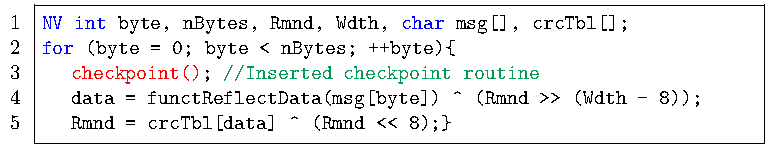
\includegraphics[width=\columnwidth]{figures/crc_example}
		\caption{Simplified C code snippet of a CRC calculation from~\cite{hicks_mibench2_2016}: per-byte message division by a polynomial; \texttt{NV} denotes non-volatile variable declaration.}\label{fig:crc_example}
	\end{subfigure}
	\begin{subfigure}[t]{\linewidth}
		\centering 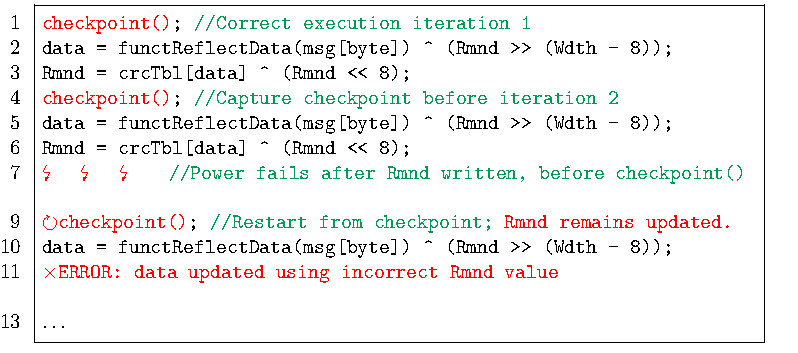
\includegraphics[width=\columnwidth]{figures/crc_example_war}
		\caption{Execution steps of the loop body in the snippet above: non-volatile checkpointing did not guarantee data consistency as data has been manipulated (line 9) with stale reminder (line 3)}\label{fig:crc_example_war}
    \end{subfigure}
	\caption{\textbf{Code example demonstrating effect of write after read on volatile memory checkpointing.}}\label{fig:code_demo_incosistency}
\end{figure}

%\begin{figure}
%	\centering
%	\subfloat[Simplified C code snippet of a CRC calculation from~\cite{hicks_mibench2_2016}: per-byte message division by a polynomial; \texttt{NV} denotes non-volatile variable declaration]{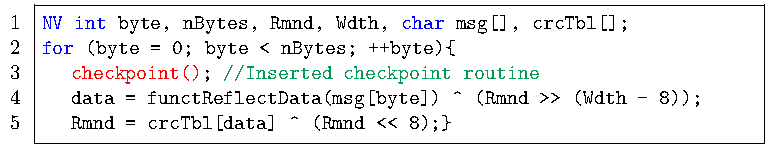
\includegraphics[width=\columnwidth]{figures/crc_example}\label{fig:crc_example}}\\
%	\subfloat[Consecutive execution steps of the loop body in the snippet above: non-volatile checkpointing did not guarantee data consistency as data has been manipulated (line 9) with stale reminder (line 3)]{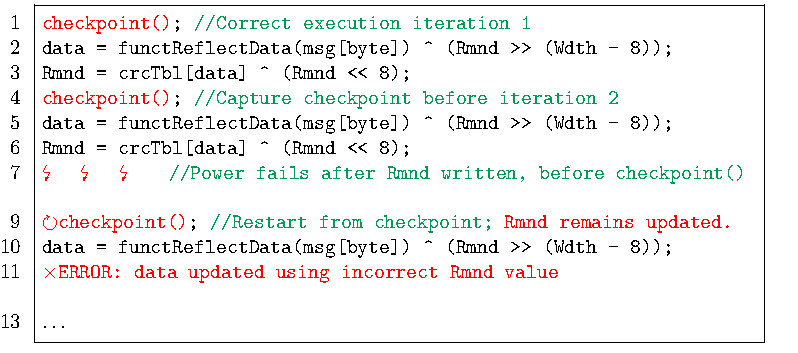
\includegraphics[width=\columnwidth]{figures/crc_example_war}\label{fig:crc_example_war}}
%	\caption{Code example demonstrating effect of write after read on volatile memory checkpointing.}
%	\label{fig:code_demo_incosistency}
%\end{figure}

Checkpoints of volatile state preserve intermittent progress, but do not ensure data consistency~\cite{dino,chain,ratchet}. Data may become inconsistent if an attempt to execute some computation {\em writes} to a non-volatile variable, then power fails, then a second attempt to re-execute the same computation incorrectly {\em reads} the value written in the first attempt, rather than the variable's original value. The situation occurs when code includes a WAR dependence between operations that manipulate non-volatile variables~\cite{ratchet,dino,alpaca}.

Figure~\ref{fig:code_demo_incosistency} illustrates how state can become inconsistent in an intermittent execution using the cyclic redundancy check (CRC) code from MIBench2~\cite{hicks_mibench2_2016}. The code computes the CRC for an $\texttt{nBytes}$ byte message $\texttt{msg}$ with remainder $\texttt{Rmnd}$.

Despite checkpointing at line 3 in Fig.~\ref{fig:crc_example}, the code may compute  $\texttt{data}$ incorrectly because of the read of $\texttt{Rmnd}$ on line 4 and the write of $\texttt{Rmnd}$ on line 5. Figure~\ref{fig:crc_example_war} shows an intermittent execution. The second iteration writes $\texttt{Rmnd}$, but power fails before the checkpoint. After restarting, line 9 reads the updated value of $\texttt{Rmnd}$, producing an incorrect $\texttt{data}$ value. Checkpoint-based systems risk violating memory consistency~\cite{dino}. To maintain consistency, prior systems~\cite{dino,ratchet} {\em version} a subset of non-volatile data with the checkpoint. Task-based systems~\cite{chain,alpaca}, which we focus on, ensure consistency using programmer, compiler, and runtime support.

\subsection{Task-based Intermittent Programming}
\label{section:background_task_computing}

Task-based execution models~\cite{dino,chain,alpaca} ask the programmer to decompose their program into tasks. A task is a function with no caller containing arbitrary computation, sensing, and communication. A programmer describes task control-flow as a {\em task graph}. Task flow happens at programmer demarcated transition points that may be conditional on program values. Task-based programming abstractions guarantee that tasks execute {\em atomically}, regardless of power failures. Task-based runtime systems ensure task-atomic semantics by ensuring that repeated task executions are idempotent. The key to idempotence is ensuring that non-volatile updates made by an interrupted task are never visible to a future task execution.  

There are several run time strategies to ensuring task idempotence. One approach~\cite{alpaca}, is to identify non-volatile data involved in WAR dependences in a task (like DINO~\cite{dino} and Ratchet~\cite{ratchet} did for checkpoints), execute the task using private copies of those data, and commit the private copies on task completion. Another way is to statically create multiple versions of non-volatile data shared by tasks and ensure that no task reads and writes the same version~\cite{chain}. Regardless of the strategy, task-based systems execute statically-defined tasks atomically, completing in one or more attempt. 

\begin{table}
	\centering
	\footnotesize
	\begin{tabular}{|c|c|}
		\hline
		Model & Data Copied to/from NVRAM \\
		\hline\hline
		Mementos~\cite{mementos}                             & Reg. + Stack     \\
		DINO~\cite{dino}                                     & Reg. + WAR variables \\
		Chain~\cite{chain}                                   & PC   + Channel data\\
		Alpaca~\cite{alpaca}                                 & PC   + WAR variables \\
		Ratchet~\cite{ratchet}, Clank~\cite{hicks_isca_2017} & Reg. (requires NV main memory) \\
		\hline
	\end{tabular}
	\caption{\textbf{Memory consistency enforcement overheads of intermittent execution models;} \emph{Reg.}: the entire register file, \emph{PC}: program counter, \emph{Channel data}: variables explicitly task-shared by the programmer, \emph{WAR variables}: variables involved in WAR dependences (\emph{NV}: non-volatile).}
	\label{table:chechpoint_comparison}
\end{table}

\subsubsection{Costs of Task-based Models}

%Task-based models incur costs that motivate \sys.

\textbf{Memory Consistency Enforcement Overhead.} Intermittent execution models incur overheads to checkpoint data~\cite{dino,ratchet,quickrecall,mementos}, manage channels~\cite{chain}, or privatize and commit data~\cite{alpaca}. Table~\ref{table:chechpoint_comparison} compares overheads for recent intermittent execution models (cf. \cite[Sec. 2.4]{alpaca}.) The mechanism responsible for overhead in each model varies, but the bulk of overhead in all models is a manipulating non-volatile memory. Checkpointing moves data to and from non-volatile memory, channel accesses manipulate non-volatile data~\cite{chain}, privatization copies from and commits to non-volatile memory~\cite{alpaca}, and idempotence solutions~\cite{ratchet} use {\em only} non-volatile memory.  

\begin{figure}
\begin{subfigure}[t]{.49\columnwidth}
	\centering 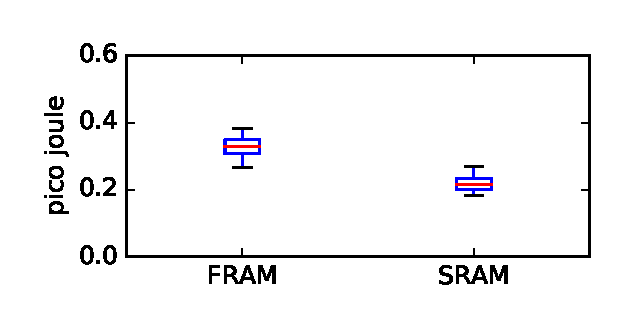
\includegraphics[width=\columnwidth]{figures/fram_write}
	\caption{Cost of \emph{write} operation}
\end{subfigure}%
\begin{subfigure}[t]{.49\columnwidth}
	\centering 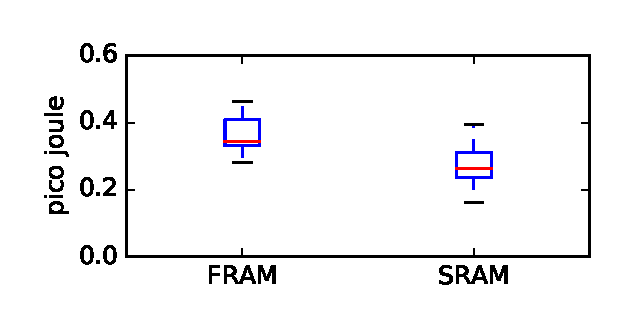
\includegraphics[width=\columnwidth]{figures/fram_read}
	\caption{Cost of \emph{read} operation}
\end{subfigure}
	\caption{\textbf{Cost of accessing volatile (SRAM)/non-volatile (FRAM) memory during write/read operation.}}\label{fig:framEnergy}
\end{figure}

%\begin{figure}
%\centering
	%\subfloat[Energy cost of \emph{write} operation]{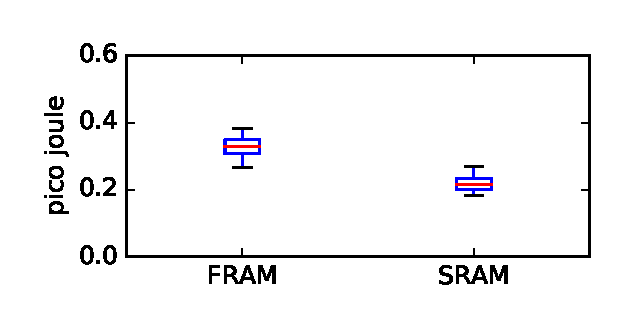
\includegraphics[width=0.49\columnwidth]{figures/fram_write.eps}}
	%\subfloat[Energy cost of \emph{read} operation]{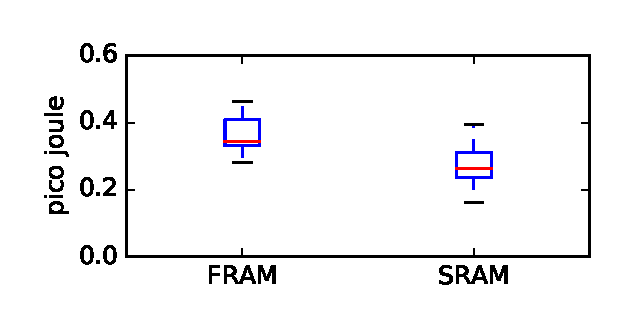
\includegraphics[width=0.49\columnwidth]{figures/fram_read.eps}}
	%\caption{Cost of accessing volatile (SRAM)/non-volatile (FRAM) memory during write (left) and read (right) operation.}
	%\label{fig:framEnergy}
%\end{figure}

To understand these non-volatile memory overheads, for the MSP430FR5969~\cite{msp430datasheet} MCU we measured the energy consumption of volatile (SRAM) and non-volatile (FRAM) memory operations. We used EDB~\cite{edb} to monitor voltage drop on a capacitor powering the device across 1600 read and write accesses to each memory type, randomizing to avoid caching. Figure~\ref{fig:framEnergy} summarizes the data, showing that a non-volatile memory access consumes around 1.5 times the energy of a volatile access in this device. In an intermittent device, energy cost corresponds to decreased run time between power failures. The cost of non-volatile memory motivates \sys, which virtualizes memory to primarily use SRAM.

%The above result reassures the intuitive observation that a decrease of checkpoint frequency (CP) decreases the energy cost associated with each state preservation method and reduces operation cost which in most simplistic terms is defined as $\mathcal{O}(\text{CP})+\mathcal{O}(\text{PL})$, where PL is the cost of program execution without checkpointing. On the other hand, this increases task/checkpoint re-execution time. The ideal solution is a runtime that \emph{adaptively} changes task size during runtime, which however exposes a second problem.

%\begin{table}
%	\centering
%	\footnotesize
%	\begin{tabular}{|c|c|}
%		\hline
%		Platform name & Storage capacitor size \\
%		\hline \hline
%		%Moo~\cite{moo} & 0.1\,F \\
%		WISPCam~\cite{naderiparizi_rfid_2015} & 6.08\,mF \\ %tested [11.24, 17.45, 21.98]\,mF
%		%NFC-WISP~\cite{zhao_rfid_2015} & 300\,$\mu$F \\
%		NeuralWISP~\cite{holleman_biocas_2008} & 100\,$\mu$F \\
%		WISP~\cite{wisp5} & 47\,$\mu$F \\
%		{\em BioImpedance} sensor~\cite{rodriguez_tbcs_2015} & 20\,$\mu$F \\
%		{\em Ingestible} sensor~\cite{nadeau_naturebio_2017} & 220\,$\mu$F\\
%		\hline
%	\end{tabular} 
%	\caption{{\em Default} energy storage sizes for example battery-less platforms. Observe a huge variation in storage capacity.}
%	%We note that values for other representative platforms~\cite{medusa_farsens_2017,talla_imwut_2017,liu_sigcomm_2013,parks_sigcomm_2014} were not reported in their respective papers.
%	\label{table:capacitor}
%\end{table}

\textbf{Fixed-size Tasks are Inflexible and Inefficient.} If a programmer writes a task that consumes {\em more} energy than the device can buffer, the task will never complete using buffered energy {\em preventing forward progress} by repeatedly re-executing. If a programmer writes tasks that consume far {\em less} energy than a device can buffer, the system may operate {\em inefficiently}. When a task and its successor both complete, the two tasks were interleaved by a task boundary that preserves progress and state (i.e., checkpoint or commit). However, absent a power failure, the work to preserve state was {\em unnecessary}, incurring overhead on the tasks' executions.

Avoiding excessively costly, non-terminating tasks and short, high-overhead tasks is a programming challenge, given fixed hardware with a fixed energy buffering capacity. Buffer sizes from prior work vary widely from 20\,$\mu $F~\cite{rodriguez_tbcs_2015} to 0.1\,F~\cite{moo}. Sizing tasks complicates {\em porting} code from one device to another. An excessively costly task on a device with a small energy buffer may be a relatively short, task on a device with a larger buffer. The key problem is that using existing systems, the programmer statically sizes tasks for a fixed energy buffer. \sys's {\em task coalescing}, described
in Section~\ref{sec:task_coalescing}, is motivated by these observations.


\section{\sysfull}
\label{sec:overeall_system}

\begin{figure}
	\centering
	%\includegraphics[width=0.25\columnwidth]{figures/}
	\caption{\sys top-level description.}
	\label{fig:}
\end{figure}

Describe the overall system, the programming model, and the semantics/execution model. This should include a discussion of memory virtualization and task coalescing.

\section{Memory Virtualization}
\label{sec:memory_virtulaization}

\begin{figure}
	\centering
	%\includegraphics[width=0.25\columnwidth]{figures/}
	\caption{Memory virtualization architecture.}
	\label{fig:}
\end{figure}

\section{Task Coalescing}
\label{sec:memory_virtulaization}

\begin{figure}
	\centering
	%\includegraphics[width=0.25\columnwidth]{figures/}
	\caption{Task coalescing architecture.}
	\label{fig:}
\end{figure}

\section{Discussion}
\label{sec:discussion}

\section{Methodology and Evaluation}
\label{sec:methodology_evaluation}

\section{Related Work}
\label{sec:related_work}

\section{Conclusions}
\label{sec:conclusions}

This paper presented \sys: \sysfull.

%%%%%

\section{Old Introduction}
	Intermittently powered devices (IPDs) are battery-less devices that utilize the ambient energy to sense, compute and, communicate. For example, Wireless Identification and Sensing platform WISP \cite{wisp} uses the RF signal power to drive its computation and communication. Because of the reliance of TPDs on intermittent power supply, the harvested energy when it is available, their programs are susceptible to a very frequent power interrupts, in the order of tens of millisconds~\cite{}. Therefore, these devices require a different software execution model that complies with the nature of a discontinuous power supply. 

	The intermittent (discontinuous) execution model defines a program execution as cumulative discrete process. The main difference between the intermittent and the conventional (or continuous) execution models is that, a power failure is seen by the continuous model as an \emph{exception} that may reset the progress of a program to its beginning. Whereas, in intermittent execution a power failure is regarded as a temporary \emph{pause} to the execution that may result in some progress degradation. Generally we can classify the intermittent execution model into: 
	\begin{itemize}
		\item \emph{Sequential Execution Model}:
			Under this model a program is seen as one big idempotent operational region that has one common context. Generally, The progress of the program is saved and updated by means of checkpointing---where all the program context (e.g. CPU registers, the stack and the global variables) is saved to a non-volatile memory. Normally, the sequential model relies on a hardware assistant to measure the voltage level in the energy reservoir to place a checkpoint~\cite{mementos, harvOS, hibernus}. The benefit of this model is that it does not require code modification by a programmer. However, it has a number of drawbacks: (i) It suffers from significant overhead \cite{chain}; (ii) the programmer should not access the non-volatile memory to guarantee the consistency of the memory~\cite{xxxx}; and (iii) it restricts the IPDs to run only a single application~\cite{inos}. 
		\item \emph{Modular Intermittent Execution Model}:
			At the heart of this model is the concept of an idempotent task. The idempotent task is C function that does not have arguments and does not return a value. This task uses a well defined interface to interact with the non-volatile memory. Therefore, it tolerates arbitrary number of power interrupts. This model, generally, produces less overhead~\cite{chain} and allows multiple applications to run on an IPD by interleaving their tasks~\cite{inos}. However, it obviously requires code modification---for example, if an algorithm is written according to the continuous execution model it has to be splitted, by a programmer, into small tasks to run under the modular intermittent execution model.
	\end{itemize}

Despite that the superiority of the Modular Intermittent Execution model, it is still a static approach that completely depends on a programmer's estimation which is mostly result in a sub-optimal code devision. Moreover, this model can only consider a single hardware configuration and it does not take environment changing into considerations. 




% Energy source


% The intermittent execution is cumulative discrete process. The intermittent execution model is only able to execute a few number of instructions, as compared to the conventional (continuous) model, before its progress is terminated. Therefore, the intermittent execution model adapts an execution progress state saving mechanism. This mechanism is realized either by means of a checkpoint~\cite{}, where all the context of the program is saved into non-volatile memory. Or 

% This progress state saving mechanism is normally injected into a program either by a compiler~\cite{}. A compiler injects trigger pointers to checkpoint (save) the context of the program into the non-volatile memory.  or it is added by a programmer~\cite{chain}. [compare these two approaches]...

% We define virtualization within the context of intermittent execution as utilizing the volatile memory instead of non-volatile when the intermittent execution model attempts to access the non-volatile memory. 

\subsection{Why not Adapting Current Approaches}
Here we highlight the challenges of adapting the state-of-the-art proposed methods to enable the execution of dynamic task sizes. 
%
%	\begin{figure}[t]
%	    \centering
%	         \subfigure[Chain: Sequential task execution flow control.]{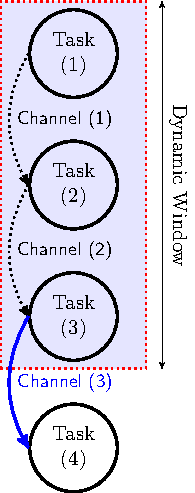
\includegraphics[width=0.35\columnwidth]{figures/dynamic-chain.pdf} \label{fig:DynamicChainSeq} } 
%	         \subfigure[Chain: Random task execution flow control.]{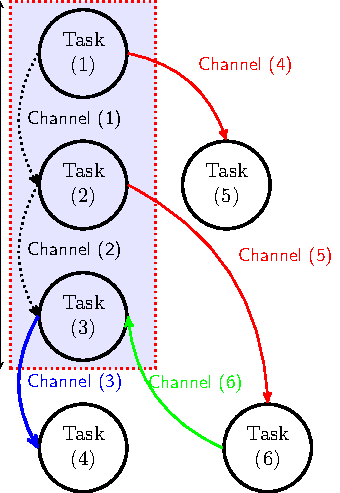
\includegraphics[width=0.61\columnwidth]{figures/dynamic-chain-2.pdf} \label{fig:DynamicChainRan}}
%	    \caption{Task flow control of Chain}
%	    \label{fig:DynamicChain}
%	\end{figure}


\noindent\textbf{Chain: Tasks and Channels for Reliable Intermittent Programs } \\
Some of the main problems in modifying Chain to support dynamic task's size are:

\begin{itemize}
	\item \emph{Multi-versioning system:} Chain defines for each task its own input that is not shared with other tasks. This design decision makes the benefit of merging tasks of less importance since each task is interacting with its own variables. 
	\item \emph{Direct FRAM system:} Chain tasks directly access FRAM which is more energy expensive Than SRAM. As result of being multi-versioning system that directly interacts with FRAM, Chain has a significant energy consumption overhead. 
	\item \emph{Irreversible tasks transitions:} According to the Chain programming model, each task calls the next one. The transition is done through functions calls and manually clearing the stack, to prevent the stack overflow problem. This approach make all the transitions firm ones which prevent task merging.
	\item \emph{All channels are required:} Fig.~\ref{fig:DynamicChainSeq} shows that if the task control flow is a circular with no branches then task merging is possible. Moreover, all the intra-merged-tasks channel can be committed to SRAM instead of FRAM to save energy. However, this execution path is only a special. If the general case (see Fig.~\ref{fig:DynamicChainRan}) is considered then leaving out the intra-merged-task channels might result in data inconsistency---If an application tries to access a merged task from the middle after a power interrupt then the input for that task is not ready which result in an incorrect execution. 


\end{itemize}


\noindent\textbf{Alpaca: Intermittent Execution without Checkpoints} \\
Some of the main problems in modifying Alpaca to support dynamic task's size are:

\begin{itemize}
	\item \emph{Privatization:} The core concept of Alpaca is privatization. Privatization depends completely on detecting the variables that have a Write-after-read dependency within the scope of a task. Therefore, if tasks are on-demand merged the scope of these dependencies are changed and the static analysis to privatize these variables is not valid anymore and data consistency can not be preserved.  

	\item \emph{Irreversible tasks transitions:} Similar to Chain problem. 

\end{itemize}

\noindent\textbf{Virtualizing Modular Intermittent Execution Model}

		An Intermittently executed program, as seen by the modular intermittent execution model, is a chain of tasks with a firm transition from one to another. 
		Virtualizing this model means softening a number of transitions, by keeping the state of the execution progress in the volatile memory, to construct a bigger \emph{virtual task} to reduce energy consumption. Ideally, the size of the virtual task should match the length of a continuous interval of the intermittent power supply for the best performance. Another form of virtualization can be achieved by reducing the number of non-volatile memory accesses. This can be done by having a temporary copy of a global variable in the volatile memory (similar to the catching principle) and a task interacts with it and updates it before writing back the most recent value to the non-volatile memory during the commit process.

		In this paper we are introducing VIPOS a runtime library the implement the Virtualed Intermittent Execution Model. VIPOS adapts two methods for data protection. One relies on a virtual buffer and the other uses the Direct Memory Access (DMA). VIPOS is able to approach the optimal tasks devision during the runtime. VIPOS reduces an application execution time by XX and the energy by XX. 


\subsection{Contributions}
	 \begin{enumerate}
		 \item We have developed an algorithm that is able to determine the size of a virtual task based on the history of the execution of an application. 
		 \item We enable efficient code portability by requiring that a real task to small and merging them during the execution.   
	\end{enumerate}


 \section{Preliminary Results}
 \label{sec:prelResults}

\begin{figure}[t]
    \centering
         \subfigure[The energy cost of FRAM/SRAM \textbf{writes} operations.]{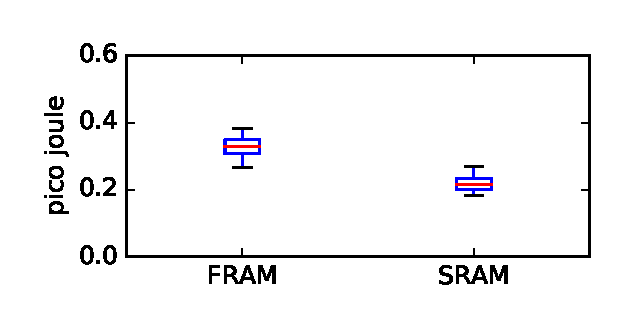
\includegraphics[width=0.48\columnwidth]{figures/fram_write.eps} }
         \subfigure[The energy cost of FRAM/SRAM \textbf{read} operations.]{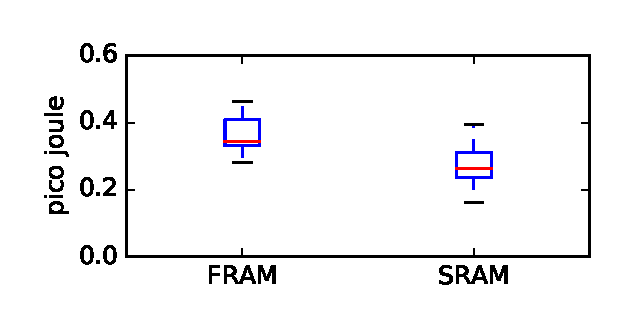
\includegraphics[width=0.48\columnwidth]{figures/fram_read.eps}}
    \caption{The energy cost of accessing volatile/non-volatile memory}
    \label{fig:framEnergy}
\end{figure}

Since the Intermittent execution models rely on the non-volatile memory to enable long-running operation, it is important to characterize the energy consumption of accessing this type of memory as compare to the volatile one.

Four applications are developed to measure the energy consumption of \emph{Accessing} the FRAM and SRAM of the MSP430FR5969 microcontroller~\cite{xxx}. The interference free debugger (EDB)~\cite{xxx} is used as the energy measurement tool. The EDB probes the energy buffer before and after accessing the FRAM/SRAM 1600 times, This large number of FRAM access is used to increase the reliability of the results generated by the used measurement tool (e.g. reducing the effect of the quantization error).  The energy buffer is charged, using the EDB, to $\approx$ 2.45 volts \textbf{only} at the beginning of the execution and of the programs. The write operations were performed by writing literal values, random numbers, to the memory. However, a read operation must be followed by a write operation, therefore, we chose to write a read value to SRAM. Fig.~\ref{fig:framEnergy} shows that an FRAM access equals $\frac{3}{2}$ SRAM access~\footnote{We would like to mentioned that TI has already mentioned in this document~\cite{xxxx} that FRAM write access is more energy expensive than SRAM write access. However, TI does not quantify the energy overhead.}. Therefore, reducing FRAM access is desirable when developing  energy limited software solution  




\section{VIPOS: Virtualized Intermittently Powered Runtime Environment}
VIPOS is runtime library that facilitates tasks navigation and preserves data/memory consistency of the IPDs. It is able, on-demand, to merge tasks to reduce the number of commits to the non-volatile memory.


\subsection{VIPOS: Data/Memory Protection Methods}

\begin{figure}[t]
	\centering
	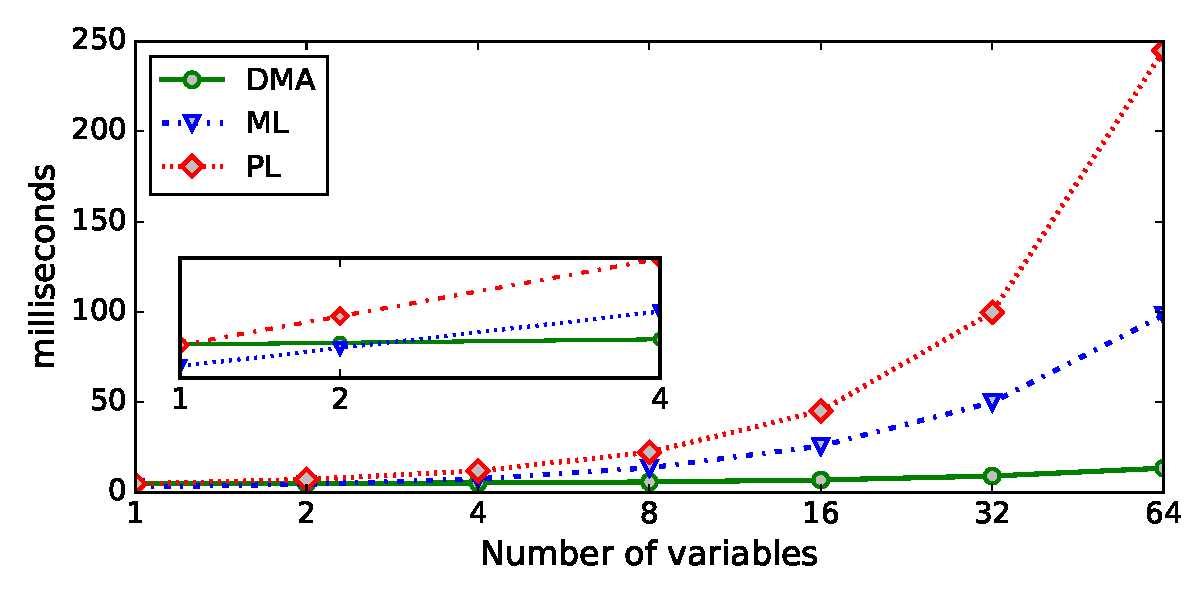
\includegraphics[width=0.8\columnwidth]{figures/iposCommitSize}
	\caption{...}
	\label{fig:virtOperationalBuf}
\end{figure}


VIPOS data consistency preservation methods are designed with goal of minimal interaction between the CPU and FRAM to reduce energy consumption (see Section~\ref{sec:prelResults}). These data/memory protection methods enables VIPOS to tolerate arbitrary number of power failures. 

	\subsubsection{Virtualized Operational Buffer}

		\begin{algorithm}[t]
			\caption{Virtualized Operational Buffer}
			\label{algo:virtuBufWrite}
			\scriptsize
			%\small
			\begin{algorithmic}[1]
				\State $var \in \text{\{global variables\}} $ 
				\State \label{lst:virtuBufWrite:line:begin}\Call{Virtual Task()}{} 
				\While { \textit{executing} } \Comment{Execution stage}
					\State $var$  $\rightarrow$ \textsf{volatile buffer} \label{lst:virtuBufWrite:line:output}
					\If { $var$  in \textsf{ volatile buffer} }				\label{lst:virtuBufWrite:line:inputBegin}
							\State $var$  $\leftarrow$  \textsf{volatile buffer} 
						\Else 
							\State $var$  $\leftarrow$  \textsf{FRAM}		\label{lst:virtuBufWrite:line:inputEnd}
						\EndIf

					\If {power interrupts}
						\State back to \ref{lst:virtuBufWrite:line:begin}
					\EndIf
				\EndWhile

				\While{  $\textsf{volatile buffer}\not=\emptyset$  } \label{lst:virtuBufWrite:line:commitBegin} \Comment{ First phase commit}
					\State \textsf{volatile buffer} $\rightarrow$  \textsf{persistent buffer}
					\If {power interrupts}
						\State discard \textsf{persistent buffer}
						\State back to  \ref{lst:virtuBufWrite:line:begin} 
						\State   \label{lst:virtuBufWrite:line:commitEnd}
					\EndIf
				\EndWhile 

				\While{ $\textsf{persistent buffer}\not=\emptyset$ } \label{lst:virtuBufWrite:line:SecCommitBegin} \Comment{Second phase commit}
					\State \textsf{persistent buffer} $\rightarrow$ FRAM 
					\If {power interrupts}
						\State Continue
					\EndIf
				\EndWhile 
				\State     \label{lst:virtuBufWrite:line:SecCommitEnd}
				\State return
			\end{algorithmic}
		\end{algorithm}


		Since accessing FRAM is more energy expensive and slower than accessing SRAM, preventing frequent access to FRAM (i.e. during looping operations) is desirable. Therefore, the first proposed protection method utilizes a volatile buffer that holds temporary all the outputs of a virtual task (see Algorithm~\ref{algo:virtuBufWrite} line~\ref{lst:virtuBufWrite:line:output}). Consequently, a virtual task must first attempt to read a global variable from the volatile buffer before trying to obtain the value from the non-volatile memory (see Algorithm~\ref{algo:virtuBufWrite} lines~\ref{lst:virtuBufWrite:line:inputBegin}-\ref{lst:virtuBufWrite:line:inputEnd}) to ensure a correct execution progress and the consistency of the memory. Once the execution of a virtual task is done, the first phase of the commit process is started by copying the volatile buffer to a persistent buffer (see Algorithm~\ref{algo:virtuBufWrite} lines~\ref{lst:virtuBufWrite:line:commitBegin}-\ref{lst:virtuBufWrite:line:commitEnd}). If the power is interrupted the persistent buffer must be discarded and the execution must start again from the beginning of the virtual task. In another words, the first phase commit must be performed atomically to preserve the consistency of the output of a virtual task. The second phase commit is a power failure immune precess that is responsible for distributing the global variables to their final locations and make the non-volatile memory consistent and synchronized with the computation progress (see Algorithm~\ref{algo:virtuBufWrite}lines~\ref{lst:virtuBufWrite:line:SecCommitBegin}-\ref{lst:virtuBufWrite:line:SecCommitEnd}).


	\paragraph{Virtualized Operational Buffer: Implementation} 

		We implement a reference implementation of VIPOS that uses virtualized Operational buffer to protect the data against power failure. 
		\paragraph{Virtual Buffer}
			We realized the virtaulzed buffer as a volatile hashed table of linked lists. The hashing technique was chosen to reduce the buffer searching time and the linked lists are used to prevent data loss when there is a conflict between multiple variables---If two variables have the same hash value they will occupy the same cell, however, with linked list a new node will be created for each variable to resolve the conflict and protect the data. The hashing function is based on the observation that the virtual addresses of the memory cells have approximately a flat distribution over the memory addressing space and the fact that each entry, of the virtual table, has the address and the value of a variable. As such, by using the least significant bits as an index to access the virtual buffer the hash function distributes its inputs uniformly in the virtual buffer. Accordingly, the linked lists search time, on average, is reduced. 

			Despite the fact that the linked lists reduce the average complexity of searching the virtual buffer significantly, they introduce a number of drawbacks: (i) the linked list data structure introduce a non-negligible memory overhead while it relies on a limited memory section, namely the heap; (ii) traversing the linked list is relatively slow. Therefore, we re-implemented the virtual buffer, after observing that most of the global variables have the same most significant bits, as a bigger hashed table that does not allow entries conflict. To eliminate the need for searching the hashed table linearly while committing its entries, we add a new buffer that holds the indices of the occupied cells of the hashed table. This table is of the same length as the hashed table. We can reason about the benefit of this buffer as follows: if we assume that the global variables are evenly divided between the tasks, then this buffer reduces the commit time by a factor equal to the number of tasks.   

		\paragraph{Persistent Buffer}
			The persistent buffer is implemented as static array of tuples, where each tuple holds  the address and the value of a variable. This data structure is very suitable for the second phase commit where each element has to be committed to its finial location. However, the complexity of committing this buffer is of size $O(N)$, where $N$ equals the length of the buffer. Therefore, the size of the buffer can have dramatic effect on the performance of VIPOS---On one hand, if the size of the buffer is small the buffer overflow problem will be very serious. On the other hand, if the size of the buffer is large VIPOS will experience a significant performance degradation. However, by observing the type of the information that this buffer holds, namely memory addresses, we can, on average, reduce the complexity of committing this buffer by defining the \emph{effective size} of the buffer to be the size of the buffer up to the first cell that holds an invalid memory address. Moreover, since this buffer is in FRAM which is much bigger than SRAM its size can be relatively big. 

		% \paragraph{Virtualized Operational Buffer: delay analysis}[initial results]

		% \begin{figure}[t]
		% 	\centering
		% 	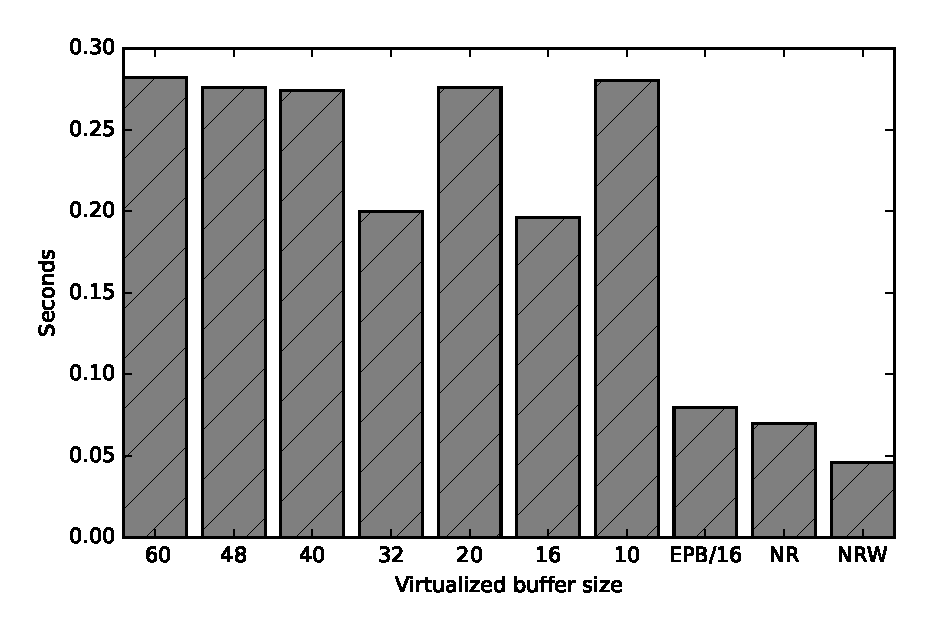
\includegraphics[width=\columnwidth]{figures/virtual_buffer_size.eps}
		% 	\caption{VIPOS based on virtualized Operational Buffer. It runs the decompression application with different buffer configurarions. EPB: Enhanced Persistent Buffer. NR: no read operation from the buffer. NRW: not read or write operations from the buffer.}
		% 	\label{fig:virtOperationalBuf}
		% \end{figure}

		% 	To analyze the performance of VIPOS versus the sizes of the virtual buffer and the persistent buffer we setup the following experiment. We let IPOS to run the decompression application---until the data decompression is completely finished---and we capture the execution time using a logic analyzer~\cite{xxx}. The results presented in Fig.~\ref{fig:virtOperationalBuf} show the VIPOS has its best performance when the virtual buffer size is 16, where the execution time was $\approx$196 ms. 

		% 	All the experiments were done with a persistent buffer of size 100. However, the bar labeled with "EPB/16" in  Fig.~\ref{fig:virtOperationalBuf} shows the effect of the enhanced commit process that uses the buffer effective size instead of the buffer maximum size. We see that the execution time is reduced to $\approx$80 ms. Furthermore, we quantized the overhead of the read operations from the buffer, by eliminating this operation, and the bar labeled with "NR" shows that it cost  $\approx$10 ms. Moreover, the overhead of the read and write operations is $\approx$34 ms as compared to VIPOS best performance, see the bar labeled with "NRW" in Fig.~\ref{fig:virtOperationalBuf}. 


\subsubsection{ Direct Memory Access Based Protection Method (better name is needed)}
%
	\begin{figure}[t]
		\centering
         \subfigure[The time needed to transfer a block of data using pointers versus Direct Memory Access (DMA).]{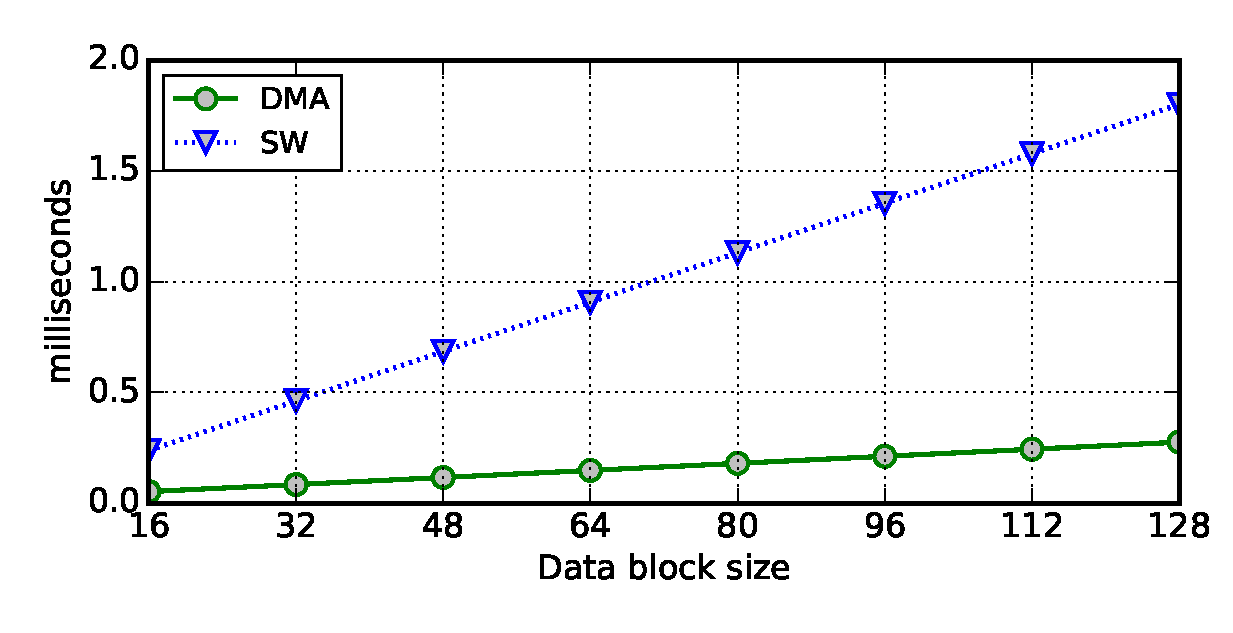
\includegraphics[width=0.48\columnwidth]{figures/dmaSize_time.eps} }
	     \subfigure[The energy needed to transfer a block of data using pointers versus Direct Memory Access (DMA).]{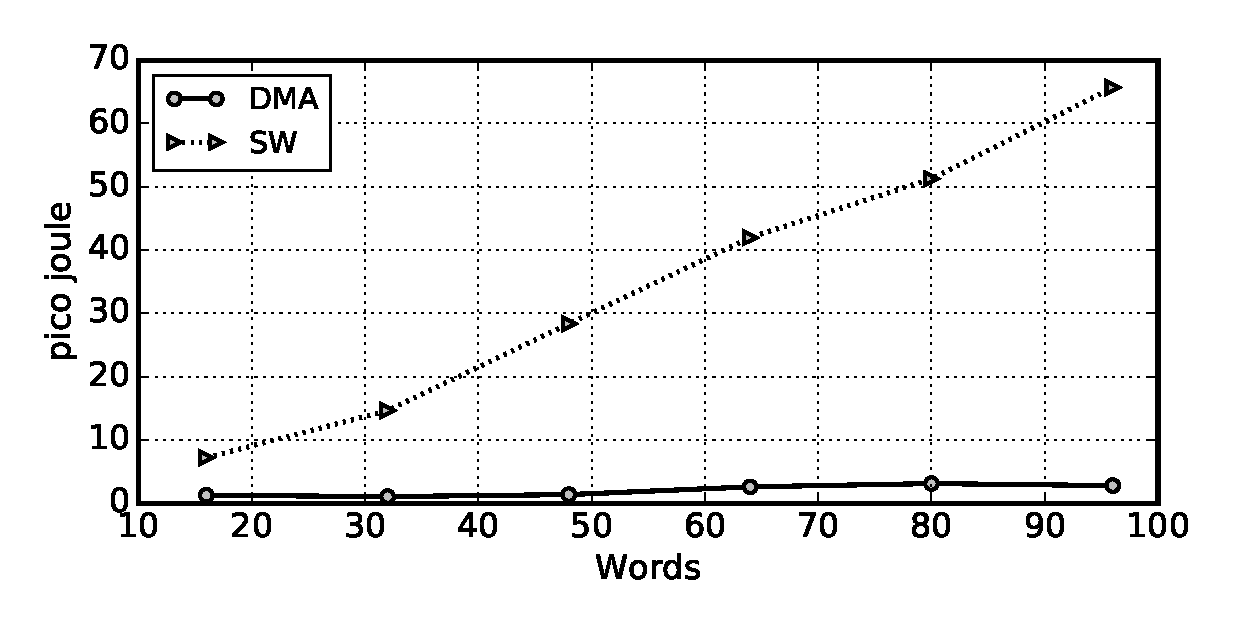
\includegraphics[width=0.48\columnwidth]{figures/energyConsumptionDMA_SW.eps}}
		\caption{Time and energy consumption of moving a block of data from SRAM to FRAM}
		\label{fig:dmaTimeEnergy}
	\end{figure}
%
	Since accessing/updating buffers is more costly than directly accessing FRAM, at least without specialized hardware~\cite{clank}, we introduce the second method to apply the virtualization principle to the Modular Execution Model. This method utilizing the Direct Memory Access (DMA) Module. As Fig.~\ref{fig:dmaTimeEnergy} shows that DMA is much more efficient in transferring a block of data than the conventional (pointer based) way from the energy and time perspectives. 

	This method combines a number of techniques to preserve the persistence and consistency of the data. It backs up the status of the global variables in the non-volatile memory, and double buffers them to guarantee their consistency. Furthermore, on each power up it populates the global variables in the volatile memory from the most recent back up in the non-volatile memory to enable a faster task execution since the task does not need to interact with non-volatile memory which is generally slower and more energy expensive.   



\subsection{VIPOS: The Virtualizing Engine}
\subsubsection{Power Interrupt Immune Scheduler}
It utilizes a persistent circular buffer (persistent linked-list) to keep the state of a program across power failures. VIPOS provides an API to enable a programmer to have a full control over the execution flow of the program, i.e. (un)blocking a task or re-execute the same task which is particularly important in the intermittent execution to emulate a persistent loop. 

\subsubsection{Task Merging Algorithms}

\paragraph{Fixed Virtual Task Size} [better name needed]

	\begin{algorithm}[t]
		\caption{Fixed virtual Task size}
		\label{algo:fixVirtTask}
		\scriptsize
		%\small
		\begin{algorithmic}[1]
			\State $VT \subset \text{\{VIPOS Tasks\}} $  \Comment{$VT:$ Virtual Task}
			\State VTS : VT size
			\State MVTS: maximum VT size
			\vspace{0.1cm}

			\While {$True$}
				\State $VT \leftarrow VT_{next}$
				\vspace{0.1cm}
				\While {execute $VT$} 
					\If { $\text{power failed twice}$ }				
							\State $VTS--$  
							\State $ MVTS = VTS $
						\EndIf
				\EndWhile

				\vspace{0.1cm}
				\If {$ \text{All tasks executed}$}
					\If{$VTS < MVTS$}
					\State $VTS++$
					\EndIf
				\EndIf
			\EndWhile
		\end{algorithmic}
	\end{algorithm}


	\begin{algorithm}[t]
		\caption{Opportunistic virtual Task size}
		\label{algo:fixVirtTask}
		\scriptsize
		%\small
		\begin{algorithmic}[1]
			\State $VT \subset \text{\{VIPOS Tasks\}} $  \Comment{$VT:$ Virtual Task}
			\State VTS : VT size
			\vspace{0.1cm}

			\While {$True$}
				\State $VT \leftarrow VT_{next}$
				\vspace{0.1cm}
				\While {execute $VT$} 
					\If { $\text{power failed twice}$ }				
							\State $VTS--$  
						\EndIf
				\EndWhile

				\vspace{0.1cm}
				\If {$ \text{All tasks executed}$}
					\State $VTS++$
				\EndIf
			\EndWhile
		\end{algorithmic}
	\end{algorithm}

\begin{figure}[t]
	\centering
	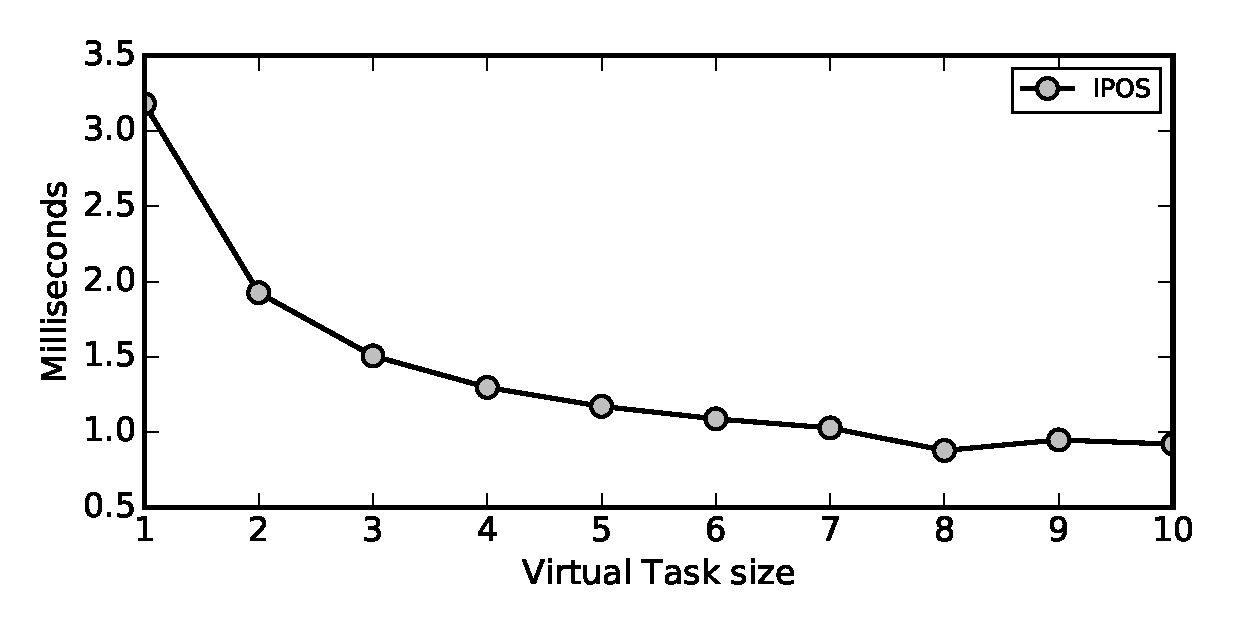
\includegraphics[width=0.8\columnwidth]{figures/virtualTaskSize.eps}
	\caption{Size of the virtual task versus the execution time of a dummy application that contains 12 empty tasks.}
	\label{fig:virtualTaskSize}
\end{figure}

VIPOS is able to virtually merge tasks to construct a bigger virtual task and commit the state of the virtual task instead of the individual real tasks. 
Fig.~\ref{fig:virtualTaskSize} show the benefit of virtualizing the Modular Intermittent Execution Mode (MIEM) in the best case scenario (continuous power supply). 

Remark: A less obvious benefit of visualization is that it can enable a secure computation. By increasing the size of the virtual task, the energy in the super-capacitor will not be enough to finish the execution of the virtual task. Therefore, without the interrogator being close to the intermittently powered device and charging rate is not negligible as compared to the discharging rate this computation will not be finished. As such, virtualization can add a layer of security to the computation.

\section{Results}
We compare the performance of VIPOS against a state-of-the-art intermittent execution approach. For this purpose, we used two different applications: (i) A data decompression application, which utilizes Huffman decoding technique to decompress 100 byte of data.; (ii) A discrete Fourier transform (DFT) application that uses two different resolution (4 and 8 bites) to analyze a randomly generated signal. 

\subsection{Continuous Power Supply}

\begin{figure}[t]
	\centering
	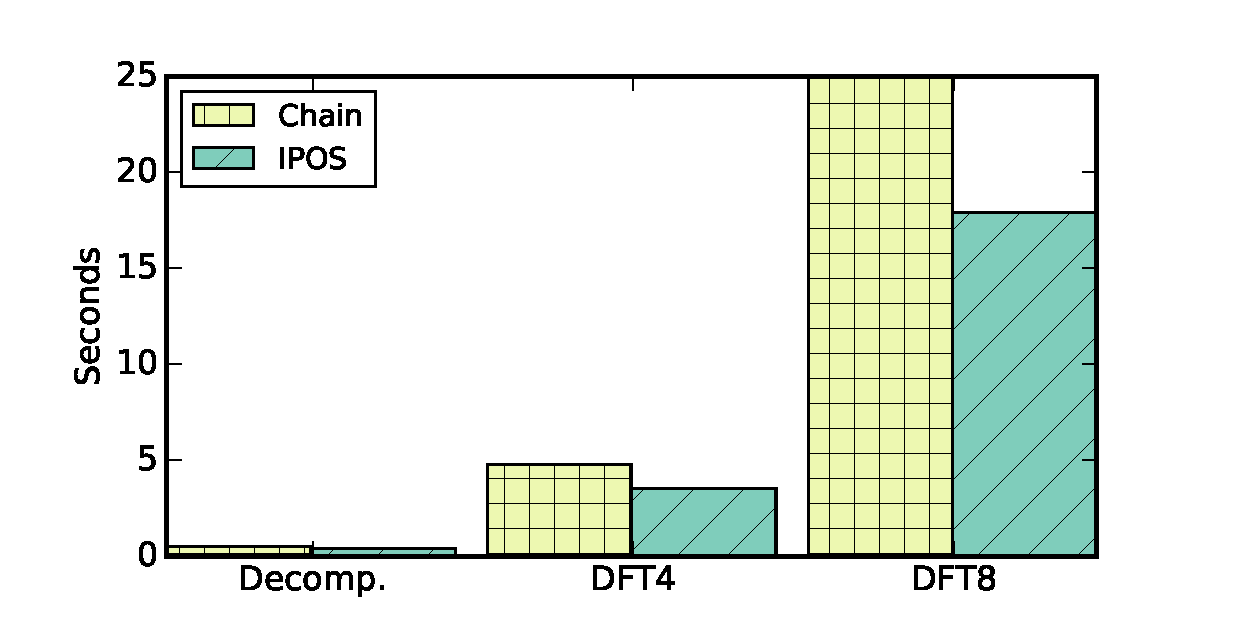
\includegraphics[width=0.8\columnwidth]{figures/ipos_chain}
	\caption{Time to complation of VIPOS versus Chain. Decomp: Data decompression application. DFTx: Discrete Fourier Transform.}
	\label{fig:IPOSPerformance}
\end{figure}

Fig.~\ref{fig:IPOSPerformance} shows that VIPOS requires a shorter execution time to execute an application under the MIEM. The size of the virtual task that VIPOS uses equals One real task, in other words, no visualization is applied.



\subsection{Intermittent Power Supply}
...

\bibliographystyle{abbrvnat}
\bibliography{bib}

\end{document}
